\chapter{Clang Analysis}

\section{Introduction}

In this chapter it will be described the analysis process for all the tools used.\newline\newline
\textbf{Understand} is indeed the tools that gives the most accurate results in terms of checks, since it incorporates C/C++ MISRA standards, a beta version of the \textbf{CLang Static Analyzer}, which is a static analysis tool provided by the LLVM developers, and many other quality checks offered by SciTools itself.\newline
A simpler but also quite effective tool is \textbf{Cppcheck} which is designed to "provide unique code analysis to detect bugs and to focus on detecting undefined behaviour and dangerous coding constructs" \cite{bibitem2}. Also, as pointed by the developers, its main focus is to  "detect only real errors in the code (i.e. have very few false positives)". Cppcheck refers to the \textsl{Common Weakness Enumeration} standard for the analysis, a formal list of security issues published by the MITRE institute. It is also possible to check MISRA-C project compliance but it requires to buy the standard so this feature was not used. \newline
The last used tool is \textbf{flawfinder} which puts its focus more on security flaws rather than quality issues. This tool incorporates an option to run the analysis in order to detect possible false positives in an automated manner. This tools uses the CWE standard as Cppcheck does.\newline
Other tools such as \textbf{SonarQube} and \textbf{Cert C Rosechecker} were used but due to their characteristics they were unusable for our purpose.
\pagebreak

\section{Understand}

Understand is a very powerful tool for static analysis that can be used to analyze software written in multiple languages suchs as Java, Ada, Cobol, Python, C/C++\dots
Among the tools used, it is the only one that comes with a nice and user-friendly user interface that allows users to navigate through the software files.\newline\newline
First of all, it must be created an \textsl{Understand Project}. In this first step you are asked to select the language of the software (C/C++ in our case study) and the directories to analyze.\newline\newline
\vspace{1cm}
\begin{minipage}{\linewidth}
	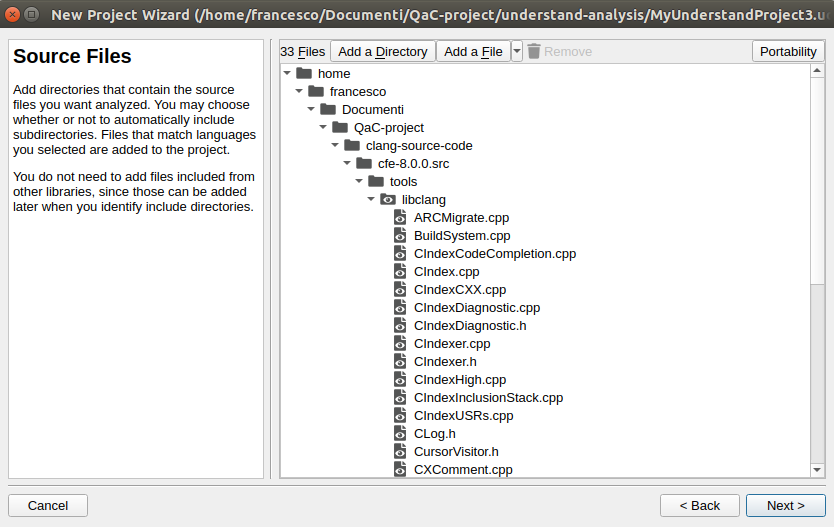
\includegraphics[width=\textwidth]{img/libclangDirectory.png}
	\captionof{figure}{The whole subdirectory tools/libclang is imported in the Understand project in order to run the analysis.}
\end{minipage}
\pagebreak

When the files are loaded in the program, the analysis can be run simply by opening the \textsl{codecheck perspective} and selecting which standard should guide it.\newline\newline
\vspace{1cm}
\begin{minipage}{\linewidth}
	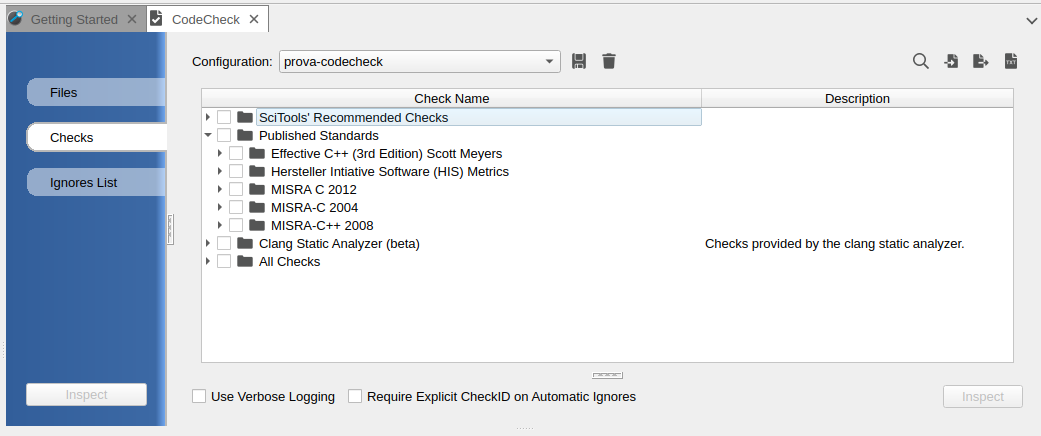
\includegraphics[width=\textwidth]{img/Codecheck.png}
	\captionof{figure}{The MISRA standard is incorporated in Understand, as well as the Clang Static Analyzer. Generic checks are also offered by the tool as \textsl{SciTools Recommended Checks} and \textsl{AllChecks}, some of which are redundant.}
\end{minipage}

\begin{itemize}
	\item \textsl{SciTools' Recommended Checks} - This is a small set (17 items) of generic good programming rules
	\item \textsl{Published Standards} - This section contains the published standards supported by Understand
		\begin{itemize}
			\item It was used the MISRA-C++ 2008 due to the nature of the source files (.cpp) and because one of the goals of this project was to check the Clang compiler compliance to MISRA rules.
		\end{itemize}
	\item \textsl{Clang Static Analyzer} - Is an implementation of the tool incorporated in Understand.
	\item \textsl{All Checks} - This is a collection of checks which consists of generic good programming rules and some of the MISRA rules. Despite its name, not all the checks are included for real, this is the reason why it is not correct to use only this option for a consistent analysis.
\end{itemize}